%\documentclass[handout]{beamer}\mode<presentation>{\usetheme{AMSCesenaPurpleAndGold}}
\documentclass[presentation]{beamer}\mode<presentation>{\usetheme{AMSCesenaPurpleAndGold}}
%%%%

\usepackage{sd-lab-process-algebra}
% \usepackage{my-listings}

\newcommand{\bs}[1]{\textbackslash{}#1}
\newcommand{\labN}{7}
\newcommand{\labGroup}{https://gitlab.com/pika-lab/courses/ds/ay2021}
\newcommand{\labRepo}{\labGroup/lab-\labN}

\title[L\labN{} -- Process Algebrae]{L\labN{} -- Modelling Distributed Systems with Process Algebrae}
%
\subtitle[SD]{Distributed Systems / Technologies}
%
\author[Ciatto \and Omicini]
{\emph{Giovanni Ciatto} \and Andrea Omicini\\
	\texttt{giovanni.ciatto@unibo.it \and andrea.omicini@unibo.it}}
%
\institute[DISI, Univ. Bologna]
{Dipartimento di Informatica -- Scienza e Ingegneria (DISI)\\\textsc{Alma Mater Studiorum} -- Universit{\`a} di Bologna a Cesena}
%
\date[A.Y. 2020/2021]{Academic Year 2020/2021}

\setbeamercovered{transparent}

\AtBeginSection{
	\begin{frame}[c]\frametitle{Outline}
		% 		\begin{multicols}{2}
		\tableofcontents[sectionstyle=show/shaded, subsectionstyle=hide/hide, subsubsectionstyle=hide/hide]
		% 		\end{multicols}
	\end{frame}
}

\AtBeginSubsection{
	\begin{frame}[c]\frametitle{Next in Line\ldots}
		\begin{multicols}{2}
			\small
			\tableofcontents[sectionstyle=show/shaded, subsectionstyle=show/shaded, subsubsectionstyle=hide/hide]
		\end{multicols}
	\end{frame}
}

\begin{document}

\maketitle

\begin{frame}[c]\frametitle{Outline}
    \begin{multicols}{2}
	    \tableofcontents[sectionstyle=show/show, subsectionstyle=show/show, subsubsectionstyle=show/show]
    \end{multicols}
\end{frame}

\section{Lecture goals} 

\begin{frame}[allowframebreaks]
    \frametitle{Lecture goals}

    \begin{itemize}
        \item Designing and implementing concurrent/distributed system (C/DS) is hard also because it is difficult to 
        %
        \begin{itemize}
            \item precisely specify the behaviour of a C/DS
            \item verify it correctly works in \alert{all possible situations}
        \end{itemize}
        
        \bigskip
        
        \item Here we will exemplify how process algebra-based modelling and reasoning may ease both a C/DS \alert{specification} -- making it clearer and more precise --, and its \alert{verification}---enabling us to prove some properties always hold (e.g. termination, deadlock-freedom, etc.)
    \end{itemize}
        
        \framebreak
        
        \begin{block}{Computer Scientist Perspective}
            Computer scientists are usually interested in proving general the \alert{correctness} of a C/DS
            %
            \begin{itemize}
                \item[eg] the PayPal payment protocol MUST be deadlock-free, and MUST guarantee a 0-or-1 semantics to payments, in ANY possibile scenario
            \end{itemize}
        \end{block}
        
        \bigskip

        \begin{block}{Software Engineer Perspective}
            Software engineers are usually interested in precisely specifying the \alert{semantics} of the software they are designing
            %
            \begin{itemize}
                \item[eg] what do you exactly mean by ``the \texttt{in} operation must suspend in case no tuple is available?''
            \end{itemize}
        \end{block}
\end{frame}

\begin{frame}%[allowframebreaks]
    \frametitle{\linda{} as a running example}

    \begin{itemize}
        \item In giving you the \linda{} specification during the previous Lab lessons, we deliberately used the natural language, often issuing \alert{ambiguous} statements on purpose
        
        \vfill
        
        \item The aim was to let you understand that several arbitrary \alert{interpretations} may be derived from an ambiguous specification
        %
        \begin{itemize}
            \item which is a nightmare for engineers
        \end{itemize}
        
        \vfill
        
        \item You should already have implemented \linda{}. We will now \alert{model} (i.e. design) it by means of CCS, transition rules, and labelled transition systems
        
        \vfill
        
        \item We will then show how several semantics could be defined from the same natural language-based specification 
    \end{itemize}
    
\end{frame}

\section{Syntax and Semantics}

\begin{frame}[allowframebreaks]
\frametitle{A workflow for semantics specification}
    
    We can \alert{formally} model a C/DS using the \href{https://en.wikipedia.org/wiki/Calculus_of_communicating_systems}{\alert{Calculus of Communicating Systems}} (CCS), and define its semantics, through the following steps:
    %
    \bigskip
    %
    \begin{enumerate}
        \item Define a \alert{syntax} for the C/DS system, covering all possible situations
        %
        \begin{itemize}
            \item this can be done by means of \alert{grammars}, which is exploited to define operators, actions, and processes
        \end{itemize}

        \bigskip
        
        \item Instantiate a particular C/DS system as a \alert{word} over the language generated by the grammar above
        
        \framebreak
        
        \item Define its semantics in terms of a \alert{Labelled Transition System} (LST), which usually implies:
        %
        \begin{enumerate}
            \item formalise the \alert{transition rules} governing the system behaviour
        
            \item adopting the aforementioned word as the \alert{initial state}
            
            \item generating the graph of possible states for the system by recursively applying all enabled transition rules to the initial state
        \end{enumerate}
        
        \bigskip

        \item Verify properties over the LTS by means of \alert{model-checkers} and \alert{temporal logics} (we won't do that) 
    \end{enumerate}
    
\end{frame}


\section{Formalising \linda{}}

\begin{frame}
\frametitle{Formalising \linda{} with process algebrae}

    We will now provide an example showing how process algebrae could be exploited to formally describe the semantics of \linda{}
    %
    \vfill
    %
    \begin{enumerate}
        \item We will model tuple spaces by means of CCS
        
        \vfill
        
        \item We will then provide their formal semantics as standalone systems, by means of a LTS
        
        \vfill
        
        \item We will model agents/users by means of CCS
        
        \vfill
        
        \item We will then provide their formal semantics as standalone systems, by means of a LTS
        
        \vfill
        
        \item Finally we will provide the syntax and the semantics of a \alert{coordinated system}, i.e., the \alert{parallel composition} of several agents/users interacting with and by means of a tuple space
    \end{enumerate}
\end{frame}

\subsection{Tuple Spaces}

\subsubsection{Syntax}

\begin{frame}
\frametitle{Tuple Spaces -- Syntax}

    \begin{block}{A grammar for \linda{'s} tuple space processes}
        \[\begin{array}{rcll}
            TS &::=& (T \cup TS) \mid (\langle T \rangle \cup TS) \mid \emptyset & \mathhint{tuple spaces}\\
            \\
            T &::=& t \mid t' \mid t'' \mid \cdots \mid t_1 \mid t'_1 \mid t''_1 \mid \cdots & \mathhint{tuples}
        \end{array}\]
    \end{block}
    
    \hint{$\langle t \rangle$ represents a tuple that is going to be inserted within the tuple space}
    
    \vfill
    
    \begin{block}{Subject to the following axioms}
        \[\begin{array}{rcll}
            X \cup Y &\equiv& Y \cup X & \mathhint{union is commutative} \\
            X \cup (Y \cup Z) &\equiv& (X \cup Y) \cup Z & \mathhint{parentheses are useless for unions}\\
            X \cup \emptyset &\equiv& X & \mathhint{neutral element for union}
        \end{array}\]
    \end{block}
\end{frame}

\begin{frame}
\frametitle{Tuple Spaces -- Several possible processes}
    
    Several tuple space processes could be syntactically represented by means of this grammar:
    %
    \vfill{}
    %
    \begin{itemize}
        \item[e.g.] $ts_0 = \emptyset$
        
        \vfill
        
        \item[e.g.] $ts_1 = t {\ \color{gray}\equiv t \cup \emptyset \equiv \emptyset \cup t \equiv t \cup \emptyset \cup \emptyset }$
        
        \vfill
        
        \item[e.g.] $ts_2 = t_1 \cup t_2 {\ \color{gray} \equiv t_1 \cup t_2 \cup \emptyset \equiv t_2 \cup t_1 \equiv t_1 \cup \emptyset \cup t_2 }$
        
        \vfill
        
        \item[e.g.] $ts_3 = t_1 \cup t_2 \cup t_3 {\ \color{gray} \equiv t_1 \cup t_2 \cup t_3 \cup \emptyset }$
        
        \vfill
        
        \item[e.g.] $ts_3 = t_1 \cup \langle t_2 \rangle \cup t_3 \cup \langle t_2 \rangle$
        
    \end{itemize}
    
    \vfill
    
    \begin{block}{}
        We say that $ts_0$, $ts_1$, $ts_2$, $ts_3$ are \alert{words} in $\mathcal{L}(TS)$, namely, the language generated by $TS$, i.e., the set of all possible tuple spaces
        %
        % Oftern, for covenience, we simply write 
    \end{block}
    
\end{frame}

\subsubsection{Semantics}

\begin{frame}
\frametitle{Tuple Spaces -- Semantics}

    \begin{block}{A grammar for tuple space related \textbf{events}}
        \[\begin{array}{rcll}
            E_{TS} &::=& !O_{TS} \mid ?I_{TS}  \mid \tau & \mathhint{event for tuple spaces} \\
            O_{TS} &::=& in(T) \mid rd(T) & \mathhint{output events} \\
            I_{TS} &::=& out(T) & \mathhint{input events} \\
        \end{array}\]
    \end{block}
    
    \pause

    \begin{block}{\linda{'s} tuple spaces as a Labelled Transition System}
        We define a tuple space $\mathcal{TS}$ as a LTS, i.e. a \emph{quartet} $ \langle S,\, s_0,\, \longrightarrow_\mathcal{TS},\, E \rangle$ where:
        %
        \begin{itemize}
            \item $S = \mathcal{L}(TS)$ is a set of possible \alert{states}
            \item $s_0 \in S$ is the \alert{initial} state
            \item $E = \mathcal{L}(E_{TS})$ is a set of event \alert{labels}
            \item $\longrightarrow_\mathcal{TS}\ \subseteq (S \times E \times S)$ is the set of admissible \alert{transitions}
        \end{itemize}
        % \[\begin{array}{rcl}
        %     TS &::=& (T \cup TS) \mid \emptyset\\
        %     T &::=& t \mid t' \mid t'' \mid \cdots \mid t_1 \mid t'_1 \mid t''_1 \mid \cdots
        % \end{array}\]
    \end{block}
    
    % \begin{block}{Subject to the following axioms}
    %     \[\begin{array}{rcll}
    %         X \cup Y &\equiv& Y \cup X & \mathhint{union is commutative} \\
    %         X \cup (Y \cup Z) &\equiv& (X \cup Y) \cup Z & \mathhint{parentheses are useless for unions}\\
    %         X \cup \emptyset &\equiv& X & \mathhint{neutral element for union}
    %     \end{array}\]
    % \end{block}
\end{frame}

\subsubsection{Transition Rules}

\begin{frame}
\frametitle{Transition Rules}

    \begin{block}{}
        The set of admissible transitions $\longrightarrow_\mathcal{TS}$ is usually \alert{intensionally} defined by means of transition rules matching the following pattern:
        %
        \[
            \frac{C_1,\ \ldots,\ C_N}{s \stackrel{e}{\longrightarrow}_\mathcal{TS} s'} \qquad [\text{RULE-NAME}]
        \]
        %
        meaning that transition $(s, e, s') \in \longrightarrow_\mathcal{TS}$ only if \alert{preconditions} $C_1$, \ldots, $C_n$ hold within the source state $s$
    \end{block}
    %
    \vfill
    %
    \begin{itemize}
        \item If no precondition of interest need to be specified, the numerator and the fraction line are usually \alert{omitted}
        
        
        \item The states $s$ and $s'$ can be represented by means of non-ground formulas containing both terminal and non-terminal symbols, i.e. variables
        %
        \begin{itemize}
            \item you can then imagine a transition rule as a \alert{rewriting rule}
        \end{itemize}
    \end{itemize}

\end{frame}

\begin{frame}
\frametitle{Tuple Spaces  -- Transition Rules}
    So, for what concerns \linda{} tuple spaces, we define the following transition rules:
    
    \[\begin{array}{rclr}
        \onslide{TS &\xrightarrow{?out(t)}_\mathcal{TS}& TS \cup \langle t \rangle & [\text{SCHEDULE}]} \\
        \\
        \onslide{TS \cup \langle t \rangle &\xrightarrow{\phantom{ab}\tau\phantom{ab}}_\mathcal{TS}& TS \cup t & [\text{INSERT}]} \\
        \\
        \onslide{TS \cup t &\xrightarrow{!in(t)}_\mathcal{TS}& TS & [\text{CONSUME}]} \\
        \\
        \onslide{TS \cup t &\xrightarrow{!rd(t)}_\mathcal{TS}& TS \cup t & [\text{OBSERVE}]} \\
    \end{array}\]
    
\end{frame}

\begin{frame}
\frametitle{Tuple Spaces  -- The state graph}
    
    \begin{columns}
        \begin{column}{.75\linewidth}
            \begin{exampleblock}{Example where $s_0 = \emptyset$}
                \href{http://www.plantuml.com/plantuml/svg/RP1FJi905CRtSuhd2ZKXAGKs3K52mMYYa5XnWomczAaJfZFDp6iKZJjDN70HkOntu2IEJ6fgxAvvl-_FrnbOueQAJ3Ax4YhdXcSmmZjUI3hLYXBnZ1065PWG9zmZMai4GLoAfQrtJtY64El223JiGQG8cEMqXXJjqeYSX5QiuhG_qV3208PykRetkb1fhAKslTvCuLFklZ3jzs6DKkf7zihO_7W1pMOVRC2ysGOHx3xUcGtylHN1YIxea8vkrJo9pyQZsSLuKOeTtMq-QRVPCjloXZ22hpUdFPyauwlhNwKx4xEXrxYE0w5yPZoT9BDB5rd2q46JUZWTkf2R2coNSngrUnmcDt-xNzNOpsfxOwUkieJjkieITkj_g0D_7pMgT7f5zv_2RwC66w1AYqn-0m00}{http://www.plantuml.com/plantuml/svg/RP1...0m00}
            \end{exampleblock}
            
            \vfill
            
            \[\begin{array}{rclr}
                TS &\xrightarrow{?out(t)}_\mathcal{TS}& TS \cup \langle t \rangle & [\text{SCHEDULE}] \\
                \\
                TS \cup \langle t \rangle &\xrightarrow{\phantom{ab}\tau\phantom{ab}}_\mathcal{TS}& TS \cup t & [\text{INSERT}] \\
                \\
                TS \cup t &\xrightarrow{!in(t)}_\mathcal{TS}& TS & [\text{CONSUME}] \\
                \\
                TS \cup t &\xrightarrow{!rd(t)}_\mathcal{TS}& TS \cup t & [\text{OBSERVE}] \\
            \end{array}\]
        \end{column}
        \begin{column}{.25\linewidth}
            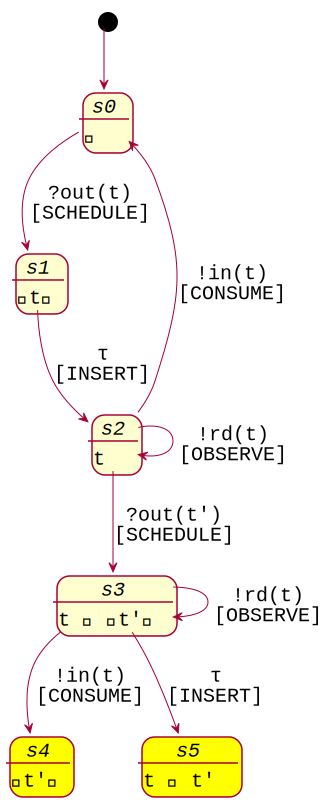
\includegraphics[width=\linewidth]{img/ts_lts.pdf}
        \end{column}
    \end{columns}
    
\end{frame}

\subsection{Users}

\subsubsection{Syntax}

\begin{frame}
\frametitle{Users -- Syntax}

    \begin{block}{A grammar for User processes}
        \[\begin{array}{rcll}
            U &::=& \mathtt{out}(T) \cdot U \mid \mathtt{in}(TT) \cdot U \mid \mathtt{rd}(TT) \cdot U & \mathhint{users} \\
            &\mid& \langle T \rangle \mid (U + U) \mid 0\\
            \\
            TT &::=& \bar{t} \mid \bar{t}' \mid \bar{t}'' \mid \cdots \mid \bar{t}_1 \mid \bar{t}'_1 \mid \bar{t}''_1 \mid \cdots & \mathhint{templates}
        \end{array}\]
    \end{block}
    %
    \hint{where $\langle t \rangle$ represent the result of an access action}
    %
    \vfill
    %
    \begin{block}{Subject to the following axioms}
        \vspace{-.4cm}
        \[\begin{array}{rcll}
            X \cdot Y &\not\equiv& Y \cdot X & \mathhint{sequence is non-commutative}\\
            X \cdot (Y \cdot Z) &\equiv& (X \cdot Y) \cdot Z & \mathhint{parentheses are useless for sequences}\\
            X \cdot 0 &\equiv& X & \mathhint{neutral element for sequences}\\
            \hline
            X + Y &\equiv& Y + X & \mathhint{choice is commutative}\\
            X + (Y + Z) &\equiv& (X + Y) + Z & \mathhint{parentheses are useless for choices}\\
            % X \cdot X &\equiv& X & \mathhint{neutral element for choices}\\
            (X + Y) \cdot Z &\equiv& X \cdot Z + Y \cdot Z & \mathhint{choice is right-distributive w.r.t sequence}\\
        \end{array}\]
    \end{block}
\end{frame}

\begin{frame}
\frametitle{Users -- Several possible processes}
    
    Several user processes could be syntactically represented by means of this grammar (not always making sense):
    %
    \vfill{}
    %
    \begin{itemize}
        \item[e.g.] $u_0 = \mathtt{in}(\bar t) \cdot \langle t \rangle \cdot \mathtt{out}(t') \cdot \mathtt{rd}(\bar{t}'') \cdot \langle t'' \rangle \cdot 0$
        \vfill
        \item[e.g.] $u_1 = \mathtt{out}(t_1) \cdot \mathtt{out}(t_2) \cdot \mathtt{out}(t_3) \cdot \mathtt{rd}(\bar t) \cdot \langle t \rangle \cdot 0$
        \vfill
        \item[e.g.] $u_2 = (\mathtt{in}(\bar{t}_1) + \mathtt{in}(\bar{t}_2) + \mathtt{in}(\bar{t}_3)) \cdot \langle t \rangle \cdot 0$
        \vfill
        \item[e.g.] $u_3 = \langle t \rangle \cdot \mathtt{in}(\bar{t}) \cdot \langle t' \rangle \cdot \mathtt{rd}(\bar{t}') \cdot 0$ \hint{makes no sense}
        \vfill
        \item[e.g.] $u_4 = \mathtt{in}(\bar{t}) \cdot \langle t \rangle \cdot \mathtt{out}(t') \cdot u_4$ \hint{recursive}
        
    \end{itemize}
    
\end{frame}

\subsubsection{Semantics}

\begin{frame}
\frametitle{Users -- Semantics}

    \begin{block}{A grammar for tuple space related \textbf{events}}
        \[\begin{array}{rcll}
            E_{U} &::=& !O_U \mid ?I_U  \mid \tau & \mathhint{events for users} \\
            O_U &::=& out(T) & \mathhint{output events} \\
            I_U &::=& rd(TT) \mid in(TT)  & \mathhint{input events} \\
        \end{array}\]
    \end{block}

    \begin{block}{\linda{'s} users as a Labelled Transition System}
        We define a user $\mathcal{U}$ as a LTS, i.e. a \emph{quartet} $ \langle S,\, s_0,\, \longrightarrow_\mathcal{U},\, E \rangle$ where:
        %
        \begin{itemize}
            \item $S = \mathcal{L}(U)$ is a set of possible \alert{states}
            \item $s_0 \in S$ is the \alert{initial} state
            \item $E = \mathcal{L}(E_{U})$ is a set of event \alert{labels}
            \item $\longrightarrow_\mathcal{U}\ \subseteq (S \times E \times S)$ is the set of admissible \alert{transitions}
        \end{itemize}
    \end{block}
\end{frame}

\subsubsection{Transition Rules}

\begin{frame}
\frametitle{Users  -- Transition Rules}
    For what concerns \linda{} users, we define the following transition rules:
    
    \[\begin{array}{rclr}
        \onslide{\mathtt{out}(t) \cdot U &\xrightarrow{!out(t)}_\mathcal{U}& U & [\text{WRITE}]} \\
        \\
        \onslide{\mathtt{rd}(\bar t) \cdot U &\xrightarrow{?rd(\bar t)}_\mathcal{U}& U & [\text{READ}]} \\
        \\
        \onslide{\mathtt{in}(\bar t) \cdot U &\xrightarrow{?in(\bar t)}_\mathcal{U}& U & [\text{TAKE}]} \\
        \\
        \onslide{\langle t \rangle \cdot U &\xrightarrow{\phantom{ab}\tau\phantom{ab}}_\mathcal{U}& U & [\text{COMPUTE}]}
    \end{array}\]
    %
    \onslide$
        \frac{U_1 \cdot U'_1 \xrightarrow{\phantom{ab}E\phantom{ab}}_\mathcal{U} U'_1}{U_1 \cdot U'_1 + U_2 \cdot U'_2 \xrightarrow{\phantom{ab}E\phantom{ab}}_\mathcal{U} U'_1} \quad [\text{CHOICE-L}]
    $ 
    \hfill
    \onslide$
        \frac{U_2 \cdot U'_2 \xrightarrow{\phantom{ab}E\phantom{ab}}_\mathcal{U} U'_2}{U_1 \cdot U'_1 + U_2 \cdot U'_2 \xrightarrow{\phantom{ab}E\phantom{ab}}_\mathcal{U} U'_2} \quad [\text{CHOICE-R}]
    $ 
    
    \vfill
    
    \begin{block}{}
        Notice that no rule exists matching state $0$ since it represents termination
    \end{block}
    
\end{frame}

\begin{frame}
\frametitle{Users -- The state graph}
    
    Example where \alert{$s_0 = \mathtt{out}(t_1) \cdot (\mathtt{rd}(\bar{t}_2) + \mathtt{in}(\bar{t}_2)) \cdot \langle t_2 \rangle \cdot \mathtt{in}(\bar{t}_3) \cdot \mathtt{rd}(\bar{t}_1) \cdot 0$}

    \begin{columns}
        \begin{column}{.70\linewidth}
            \small
            \[\begin{array}{rclr}
                \mathtt{out}(t) \cdot U &\xrightarrow{!out(t)}_\mathcal{U}& U & [\text{WRITE}] \\
                \\
                \mathtt{rd}(\bar t) \cdot U &\xrightarrow{?rd(\bar t)}_\mathcal{U}& U & [\text{READ}] \\
                \\
                \mathtt{in}(\bar t) \cdot U &\xrightarrow{?in(\bar t)}_\mathcal{U}& U & [\text{TAKE}] \\
                \\
                \langle t \rangle \cdot U &\xrightarrow{\phantom{ab}\tau\phantom{ab}}_\mathcal{U}& U & [\text{COMPUTE}]
            \end{array}\]
            %
            \[
                \frac{U_1 \cdot U'_1 \xrightarrow{\phantom{ab}E\phantom{ab}}_\mathcal{U} U'_1}{U_1 \cdot U'_1 + U_2 \cdot U'_2 \xrightarrow{\phantom{ab}E\phantom{ab}}_\mathcal{U} U'_1} \quad [\text{CHOICE-L}]
            \]
            %
            \[
                \frac{U_2 \cdot U'_2 \xrightarrow{\phantom{ab}E\phantom{ab}}_\mathcal{U} U'_2}{U_1 \cdot U'_1 + U_2 \cdot U'_2 \xrightarrow{\phantom{ab}E\phantom{ab}}_\mathcal{U} U'_2} \quad [\text{CHOICE-R}]
            \]
        \end{column}
        \begin{column}{.30\linewidth}
            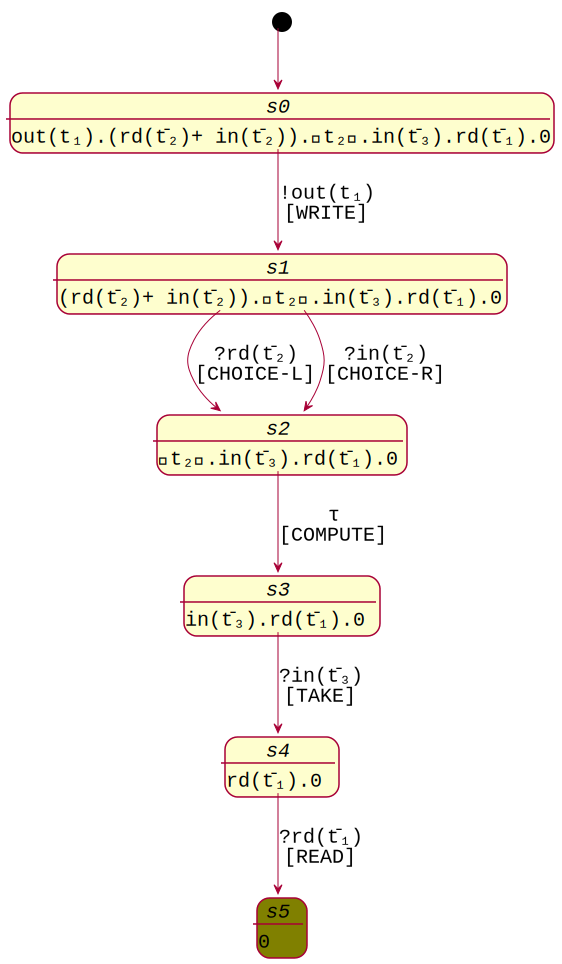
\includegraphics[width=\linewidth]{img/user.pdf}
            
            \hint{Zoomable image \href{http://www.plantuml.com/plantuml/svg/fPBDJl9058RtSnNdsz7Fq9G2cuOWM6ea_c3uYGjaCQ4ZJfZEDDEfYiQ5m98RqMinyHvw9GusjIN1nCJTIUTzdlTCCwr8OQdYWA5eJdc89GwWGsvmpDInu6f07mdOLk5meB0YNqTgmGXGXHcTHllf2nmGS4KiAP7eble4I12g1VWacaeQAYeuAf3HLWrF2E08J-SpAMBkku89sMXutATyrco2OFIEx4kCE7a8zKHydLeGniGzUaPe_7y2vN8J8Wkb-iXoGCIgf9BbYs6Mf5zIx-jakJGEWF9iDinaywhqb6pUpEppoZ2pj2QrpqhD5GV-VHkl-VYgtnrw4vJrLS21FzLKqXhRWSDSetlSarxNzSfdavr8RiyZ_NmR6npuJQcT6giEVAotejxvvQXugwhs_0XNKxXMM6UrNMVOFYqeQbgnozLIhfxVDFsZVQ_ToRawvE_10GkX5k5-7B1F}{here}}
        \end{column}
    \end{columns}
    
\end{frame}

\subsection{Coordinated Systems}

\subsubsection{Syntax}

\begin{frame}
\frametitle{Coordinated Systems -- Syntax}

    \begin{block}{A grammar for coordinated systems}
        \[\begin{array}{rcll}
            CS &::=& US \parallel TS & \mathhint{coordinated system}\\
            US &::=& (U \parallel US) \mid 0 & \mathhint{list of users}
        \end{array}\]
    \end{block}
    
    \vfill
    
    \begin{block}{Subject to the following axioms}
        \[\begin{array}{rcll}
            X \parallel Y &\not\equiv& Y \parallel X & \mathhint{parallel is \alert{not} commutative} \\
            X \parallel (Y \parallel Z) &\equiv& (X \parallel  Y) \parallel Z & \mathhint{parentheses are useless for parallel} \\
            X \parallel 0 &\equiv& X & \mathhint{neutral element for parallel}
        \end{array}\]
    \end{block}
    %
    \hint{A non-commutative parallel operator makes the processes identifiable by means of their \emph{index}}
    
    \vfill
    
    \begin{block}{}
	    Notice that the states of a coordinated systems must match the patterns:
	    %
	    \[\begin{array}{c}
	        U_1 \parallel \cdots \parallel U_i \parallel \cdots \parallel U_n \parallel TS\\
	        US \parallel U_i \parallel US' \parallel TS
	 	\end{array}\]
    \end{block}
    
\end{frame}

\subsubsection{Semantics}

\begin{frame}
\frametitle{Coordinated Systems -- Semantics}

    \begin{block}{A grammar for coordinated systems related \textbf{events}}
        \[\begin{array}{rcll}
            E_{CS} &::=& out(T) \mid in(T) \mid rd(T) \mid \tau & \mathhint{events} \\
        \end{array}\]
    \end{block}
    
    \vfill

    \begin{block}{Coordinated systems as a Labelled Transition System}
        We define a user $\mathcal{CS}$ as a LTS, i.e. a \emph{quartet} $ \langle S,\, s_0,\, \longrightarrow_\mathcal{CS},\, E \rangle$ where:
        %
        \begin{itemize}
            \item $S = \mathcal{L}(CS)$ is a set of possible \alert{states}
            \item $s_0 \in S$ is the \alert{initial} state
            \item $E = \mathcal{L}(E_{CS})$ is a set of event \alert{labels}
            \item $\longrightarrow_\mathcal{CS}\ \subseteq (S \times E \times S)$ is the set of admissible \alert{transitions}
        \end{itemize}
    \end{block}
\end{frame}

\subsubsection{Transition Rules}

\begin{frame}
\frametitle{Coordinated Systems -- Transition Rules I}

    For what concerns coordinated systems, we define the following transition rules (pay attention to the \alert{indexes} in rules names):
    
    \onslide\[
        \frac{
            \mathtt{out}(t) \cdot U_i \xrightarrow{\highlightG{!out(t)}}_\mathcal{U} U_i 
            \qquad
            TS \xrightarrow{\highlightG{?out(t)}}_\mathcal{TS} TS \cup \langle t \rangle 
        }{
            US \parallel \highlightR{\mathtt{out}(t) \cdot U_i} \parallel US' \parallel \highlightB{TS}
            \xrightarrow{\highlightG{out(t)}}_\mathcal{CS}
            US \parallel \highlightR{U_i} \parallel US' \parallel \highlightB{TS \cup \langle t \rangle}
        } 
        \quad 
        [\text{OUT}_i]
    \]
    
    \onslide\[
		\frac{
			\mathtt{in}(\bar t) \cdot U_i \xrightarrow{\highlightG{?in(\bar t)}}_\mathcal{U} U_i 
			\qquad
			TS \cup t \xrightarrow{\highlightG{!in(t)}}_\mathcal{TS} TS
			\qquad
			t \in \bar{t}
		}{
			US \parallel \highlightR{\mathtt{in}(\bar t) \cdot U_i} \parallel US' \parallel \highlightB{TS \cup t}
			\xrightarrow{\highlightG{in(t)}}_\mathcal{CS}
			US \parallel \highlightR{\langle t \rangle \cdot U_i} \parallel US' \parallel \highlightB{TS}
		} 
		\quad 
		[\text{IN}_i]
	\]
	
	\onslide\[
		\frac{
			\mathtt{rd}(\bar t) \cdot U_i \xrightarrow{\highlightG{?rd(\bar t)}}_\mathcal{U} U_i 
			\qquad
			TS \cup t \xrightarrow{\highlightG{!rd(t)}}_\mathcal{TS} TS \cup t
			\qquad
			t \in \bar{t}
		}{
			US \parallel \highlightR{\mathtt{rd}(\bar t) \cdot U_i} \parallel US' \parallel \highlightB{TS \cup t}
			\xrightarrow{\highlightG{rd(t)}}_\mathcal{CS}
			US \parallel \highlightR{\langle t \rangle \cdot U_i} \parallel US' \parallel \highlightB{TS \cup t}
		} 
		\quad 
		[\text{RD}_i]
	\]

\end{frame}

\begin{frame}
\frametitle{Coordinated Systems -- Transition Rules II}
	%
	\[
		\frac{
			\langle t \rangle \cdot U_i \xrightarrow{\highlightG{\phantom{ab}\tau\phantom{ab}}}_\mathcal{U} U_i 
		}{
			US \parallel \highlightR{\langle t \rangle \cdot U_i} \parallel US' \parallel TS
			\xrightarrow{\highlightG{\phantom{ab}\tau\phantom{ab}}}_\mathcal{CS}
			US \parallel \highlightR{U_i} \parallel US' \parallel TS
		} 
		\quad 
		[\text{COMPUTE}_i]
	\]
	\vfill
	\[
		\frac{
			TS \cup \langle t \rangle \xrightarrow{\highlightG{\phantom{ab}\tau\phantom{ab}}}_\mathcal{TS} TS \cup t
		}{
			US \parallel \highlightB{TS \cup \langle t \rangle}
			\xrightarrow{\highlightG{\phantom{ab}\tau\phantom{ab}}}_\mathcal{CS}
			US \parallel \highlightB{TS \cup t}
		} 
		\quad 
		[\text{INSERT}]
	\]
	\vfill
	\[
		\frac{
			U_i + U'_i \xrightarrow{\highlightG{\phantom{ab}E'\phantom{ab}}}_\mathcal{U} U''_i 
			\qquad
			TS \xrightarrow{\highlightG{\phantom{ab}E''\phantom{ab}}}_\mathcal{TS} TS'
			\qquad
			E = \gamma(E', E'')
		}{
			US \parallel \highlightR{U_i + U'_i} \parallel US' \parallel \highlightB{TS}
			\xrightarrow{\highlightG{\phantom{ab}E\phantom{ab}}}_\mathcal{CS}
			US \parallel \highlightR{U''_i} \parallel US' \parallel \highlightB{TS'}
		} 
		\quad 
		[\text{CHOICE}_i]
	\]
	%
	where the partial funtion $\gamma(\cdot, \cdot)$ is defined as follows:
	%
	\begin{multicols}{2}\begin{itemize}
			\item $\gamma(!out(t), ?out(t)) = out(t)$
			\item $\gamma(?in(\bar t), !in(t)) = in(t)$
			\item $\gamma(?rd(\bar t), !rd(t)) = rd(t)$
	\end{itemize}\end{multicols}
\end{frame}

\begin{frame}
\frametitle{Example: Out-In-Rd, \emph{unordered}}
    Example where \alert{$s_0 = \mathtt{out}(t) \cdot 0 \parallel \mathtt{in}(\bar t) \cdot 0 \parallel \mathtt{rd}(\bar t) \cdot 0 \parallel \emptyset$}
    
    \begin{center}
        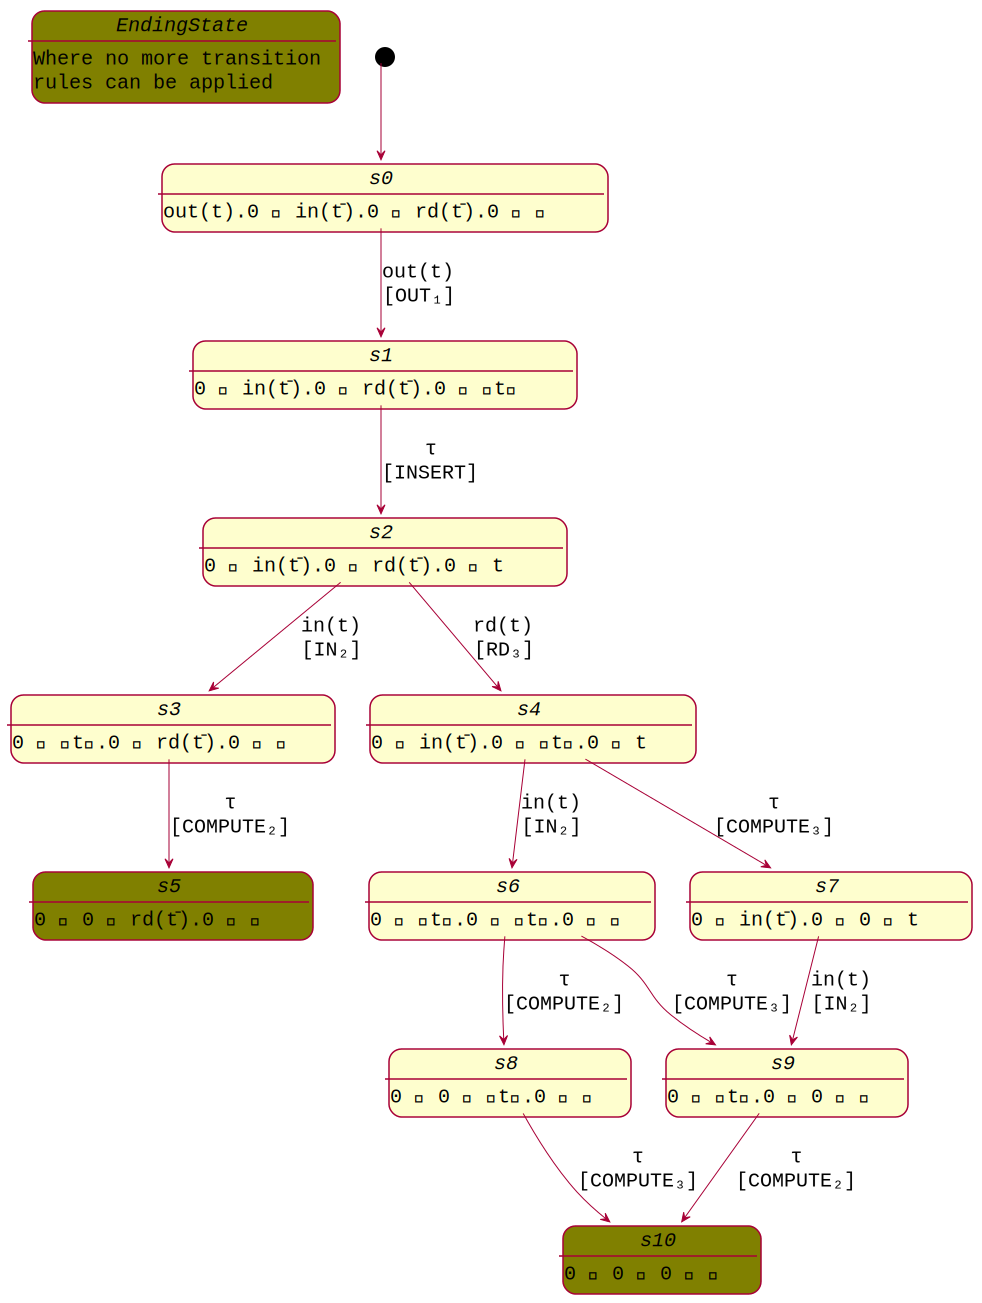
\includegraphics[width=.4\linewidth]{img/out_in_rd.pdf}
        
        \hint{Zoomable image \href{http://www.plantuml.com/plantuml/svg/ZP9FRXCn5CRtFiLRjaX5apJDdr4LLQH1Oa6BcbGisYnCvj5QzTWZ-mrIGIm8HMBHQx20io1nXpa9at7TcE1KMMJXV7w_z_kiERB43PMvPFP6g88RdiCnlkUbf9TQqKHyH6WdGJWXJjX4T2iH174fvZO-VS9pX94kZK33haM6W7b1jv2XdHjHaD2A1PDsYOPF3E05dzzS6LsgRAIbDeU7OvK9TJKSWfRY0xBFZBdBxl_62LQtKdXxZGP1QSYrGI33bHNBTPVAb18jpBc2TmYyAAJ0ZB6BPpFOsnk2JHx0Dab1bxH3kyyJgBx_0A5swFUTFvaiEDM_Rymc3j3oSvVgulHyMYs-pBpiCji2Tl-JgljVpBOSi9t2dxiQzkfaCZwRhc3jRM34RDjXzjFcucv3gXQBsMFIIUiXbvmTLuklVaKpyu_JvlBx3dNmu3ewVVtcV3fkrdXO9-gxGdlVZaDr__FrIMzzIM1y47m5VjycQJ_JZRSCJhvbrmdq8orzDdX2hXT_WSVcFOzOR-u1VG_OQDXtY5RoXCOWtZUW3EAKqAKEOq-zHZf2bPMv_0i0}{here}}
    \end{center}
\end{frame}

\startExercise

\subsection{Out-Out-In-In, \emph{unordered}}

\begin{frame}[allowframebreaks]
\frametitle{Exercise \currentExercise{} -- Out-Out-In-In, \emph{unordered}}
    \begin{enumerate}
        \item Clone the Lab \labN{} GitLab repository: \url{\labRepo}
        
        \vfill
        
        \item Consider the system with \alert{$s_0 = \mathtt{out}(t_1) \cdot \mathtt{out}(t_2) \cdot \mathtt{in}(\bar t) \cdot \mathtt{in}(\bar t) \cdot 0  \parallel \emptyset$}, where $t_1, t_2 \in \bar{t}$, s.t. the \linda{} semantics defined before
        
        \vfill
    
        \item Complete the state graph according to the transition ruled defined before and include the state graph image in your \alert{\texttt{README.md}} file
        %
        \begin{itemize}
            \item web editor here: \href{
                http://www.plantuml.com/plantuml/uml/ZPBVJl8m6CRFUnNl8Nm9P8m_4488-H0JJp0HE48E6bQneMkNjLFHUE22YGVSXWToBIRU0rTYHvakSpWFbhNls-VtF6_JdbJOLu7Ba5nIxc4Vkt12hd30rAdWQaJl2TXMeZbIM95zIwqO0QemetEPhHvYbq1V13ubFhgc3W7YUce53f5pdtgA2euIIXcXuG41_CVpvS8N0NVwWWc_qnbmX_95jmk2qHkITMB2oPsdLyJHfrQ4CN6B7X6Q_fj1gTG5QI63brORHA0AQXS-5Sk7LLWiKrvGx-lllmMxbrVzFIDf6K8b8Rpaq_F9MAzco71DEu-sUOlKkyqMoOg1sctuM6lQsN0qk1ZFlkhL12t3p8PyjyWAITlmQl0xiAhxUQ7rTdlOXliPgWTsQeQuNa_LZPV9SZpo3vUQeJMCoDo-PkxZnytc4QlwNyUAt92iPzFYUYkE42OYn5ODI3t2Ti8ZqzoCPzJDj3hlYapYMDxADZSUnrzXZt0dSDad
            }{\texttt{http://www.plantuml.com/plantuml/uml/ZP...SDad}}
        \end{itemize}
        
        \vfill
        
        \item On the state graph, edges' labels should show both:
        %
        \begin{itemize}
            \item the event raised by the transition
            \item the transition rule justifying the edge
        \end{itemize}
        
        \vfill
        
        \item You can rely on the tools listed on slide \ref{useful-tools} for your exercise
        
        \vfill
        
        \item Commit \& push your \texttt{README.md} file
        
    \end{enumerate}
    
    \framebreak

    \begin{center}
        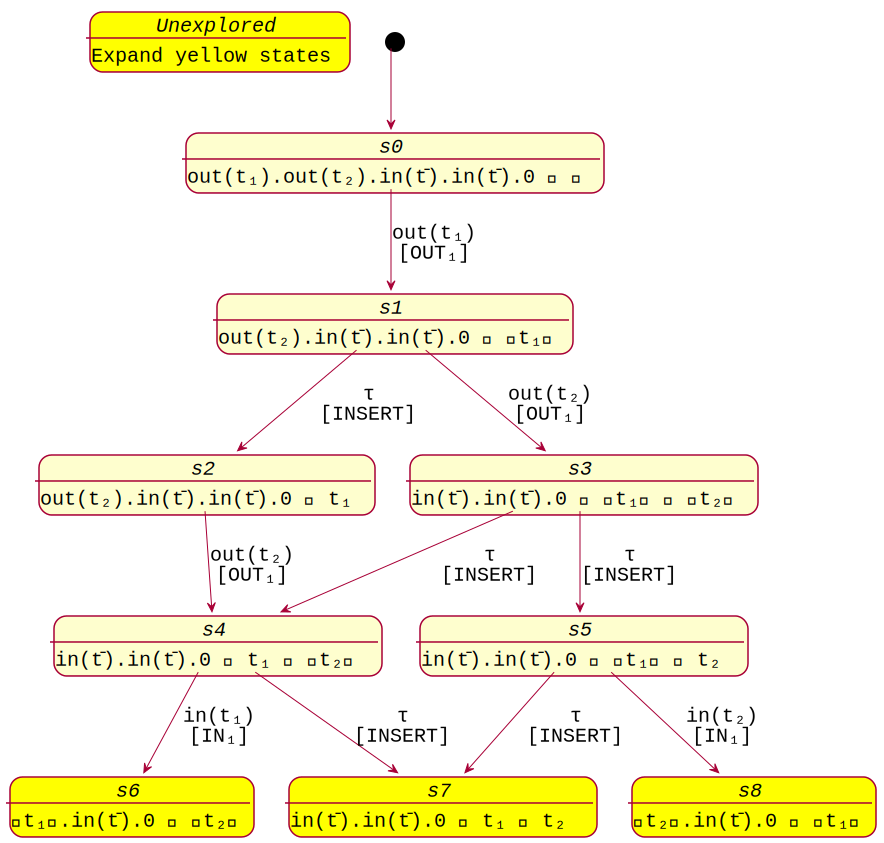
\includegraphics[width=.5\linewidth]{img/ex1.pdf}
    \end{center}
    %
    \hint{Zoomable image \href{http://www.plantuml.com/plantuml/svg/ZPBFpj905CNtynHt-Nqca5B-G1f2Y8Y96qm4LiXYGaUSC9rfEbC5ZGiRJ5pm6YxaMKny1vx4ARULMejrGRYzTyxld3kPiJOqCd4WYDvn6TA81l2ClQ6nCC-LD7F-WO7h58PpGmsxZin1CE262hxHrUeP3HXCL1nn5f6tt6V0Wj0Sm6Tw4_7GS2L9GQbJD7ma04_fPhUDL2pzYH8g6WwdqkToEng14lmTgpgnb6mVsehvzjI12Q7Uaq-48FCsX3zFUZ3TXrJwcG8ZQ49MJzRGQ8n0EqYmXGSgDW_cadn-R6PLyjZayi7yEDx-7RXy_MP_NuXsaD0g25_BrSlbmbRhB1cEwsYdxwdwSZeJtKAewy7FewMzcCsdhnRht_tsZLPbvaAzMsf5j8ky3lmRsBRpkj3syvnz9jSTsXcxj4FUxvRww8LPxaV-owM3j1wAyFOjyne_7_RlM7N_TwtKZUXkDItl3_88II52RjM3qjlr2XwLvhWUgljbTTqLOU9SFgWsHu_xht3Cf1y7uXS0}{here}}
\end{frame}

\section{\linda{} Semantics}

\begin{frame}
\frametitle{Ordered VS Unordered Semantics for \linda{}}

    \begin{itemize}
        \item The tuple space semantics defined so far is known as the \alert{unordered} semantics of \linda{}
        %
        \begin{itemize}
            \item long story short: if $n$ tuples are orderly \texttt{out}'d by an agent, you cannot assume them to be inserted into the tuple space in the same order
            \begin{itemize}
                \item[$\implies$] agents cannot use tuple spaces as counters $\implies$ \alert{no Turing equivalence}
            \end{itemize}
        \end{itemize}
        
        \vfill
        
        \item Unordered semantics $\implies$ the \texttt{out} operation is \emph{asynchronous}
        %
        \begin{itemize}
            \item \texttt{out}ing agents resume execution before tuples are actually inserted
        \end{itemize}
        
        \vfill
        
        \item We now provide an \alert{ordered} semantics where the \texttt{out} primitive is \emph{synchronous}, and the resulting coordinated system is Turing-complete
    \end{itemize} 

\end{frame}

\subsection{Ordered semantics}

\begin{frame}
\frametitle{Ordered semantics for \linda{}}

    \begin{enumerate}
        \item Imagine the syntax for tuple spaces was defined without a means for expressing pending tuples to be inserted:
        %
        \[\begin{array}{rcl}
            TS &::=& (T \cup TS) \mid \emptyset
        \end{array}\]
        
        \vfill
        
        \item Then, imagine transition rule $[\text{INSERT}]$ was never defined, neither for $\mathcal{TS}$ nor for $\mathcal{CS}$
        
        \vfill
        
        \item Then, imagine transition rule $[\text{SCHEDULE}]$ was defined in the following way for $\mathcal{TS}$:
        %
        \[\begin{array}{rcl}
            TS &\xrightarrow{?out(t)}_\mathcal{TS}& (TS \cup t)
        \end{array}\]
        
        \vfill
        
        \item Finally, imagine transition rule $[\text{OUT}_i]$ was defined in the following way for $\mathcal{CS}$:
        %
        \[
            \frac{
                \mathtt{out}(t) \cdot U_i \xrightarrow{\highlightG{!out(t)}}_\mathcal{U} U_i 
                \qquad
                TS \xrightarrow{\highlightG{?out(t)}}_\mathcal{TS} TS \cup t 
            }{
                US \parallel \highlightR{\mathtt{out}(t) \cdot U_i} \parallel US' \parallel \highlightB{TS}
                \xrightarrow{\highlightG{out(t)}}_\mathcal{CS}
                US \parallel \highlightR{U_i} \parallel US' \parallel \highlightB{TS \cup t }
            }
        \]
    \end{enumerate}

\end{frame}

\startExercise

\subsection{Out-Out-In-In, \emph{ordered}}

\begin{frame}[allowframebreaks]
\frametitle{Exercise \currentExercise{} -- Out-Out-In-In, \emph{ordered}}
    \begin{enumerate}
        \item Go on working on your local clone of the Lab \labN{} GitLab repository
        
        \vfill
        
        \item Consider the system with \alert{$s_0 = \mathtt{out}(t_1) \cdot \mathtt{out}(t_2) \cdot \mathtt{in}(\bar t) \cdot \mathtt{in}(\bar t) \cdot 0  \parallel \emptyset$}, where $t_1, t_2 \in \bar{t}$, s.t. the \alert{ordered} \linda{} semantics defined before
        
        \vfill
    
        \item Complete the state graph according to the transition ruled defined before and include the state graph image in your \alert{\texttt{README.md}} file
        %
        \begin{itemize}
            \item web editor here: \href{
                http://www.plantuml.com/plantuml/uml/XO_1IiD048RlynHpR8MMjCTIacBLenvgJxM79JlMePlTi3khHl5WKV15V1kVeazYQeH627XOzeV__pwOMH3b9HO6mfPjgRmgy8nkLJHouQmi-8bmdBJAXIYXdqegGyYY3EUXcxvK1U7SHS_auOur8HMbLAWfv9vBOMUXHOQ36fy1yLJbsurtqUgvCyvFf-TMizsaAJh3zzIrM5fwBEj4kbvLP8nxW1U0rSaQ1uCKGmADFYGJT55wij-zzeU_QTSVikt9rzlnJt3_yLc_TmX9OnYrm1kxkbfUrsaDZRUf_x4TK0YZHZS-xhjqO_nxqmIpB8CPMHqBymq0
            }{\texttt{http://www.plantuml.com/plantuml/uml/XO...q0}}
        \end{itemize}
        
        \vfill
        
        \item On the state graph, edges' labels should show both:
        %
        \begin{itemize}
            \item the event raised by the transition
            \item the transition rule justifying the edge
        \end{itemize}
        
        \vfill
        
        \item You can rely on the tools listed on slide \ref{useful-tools} for your exercise
        
        \vfill
        
        \item Commit \& push your \texttt{README.md} file
        
    \end{enumerate}
    
    \framebreak

    \begin{center}
        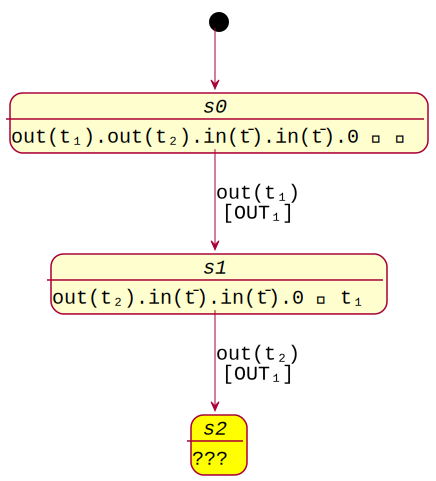
\includegraphics[width=.4\linewidth]{img/out-out-in-in.pdf}
    \end{center}
    %
    \hint{zoomable image \href{http://www.plantuml.com/plantuml/svg/XO_1IiD048RlynHpR8MMjCTIacBLenvgJxM79JlMePlTi3khHl5WKV15V1kVeazYQeH627XOzeV__pwOMH3b9HO6mfPjgRmgy8nkLJHouQmi-8bmdBJAXIYXdqegGyYY3EUXcxvK1U7SHS_auOur8HMbLAWfv9vBOMUXHOQ36fy1yLJbsurtqUgvCyvFf-TMizsaAJh3zzIrM5fwBEj4kbvLP8nxW1U0rSaQ1uCKGmADFYGJT55wij-zzeU_QTSVikt9rzlnJt3_yLc_TmX9OnYrm1kxkbfUrsaDZRUf_x4TK0YZHZS-xhjqO_nxqmIpB8CPMHqBymq0}{here}}

\end{frame}

\startExercise

\subsection{Non-deterministic Choice, \emph{ordered}}

\begin{frame}[allowframebreaks]
\frametitle{Exercise \currentExercise{} -- Non-deterministic Choice, \emph{ordered}}
    \begin{enumerate}
        \item Go on working on your local clone of the Lab \labN{} GitLab repository
        
        \vfill
        
        \item Consider the system with \alert{$s_0 = (\mathtt{out}(t_1) + \mathtt{out}(t_2)) \cdot \mathtt{rd}(\bar{t}_3) \cdot 0 \parallel \mathtt{in}(\bar{t}_4) \cdot 0 \parallel (\mathtt{in}(\bar{t}_2) \cdot \mathtt{out}(t_3) + \mathtt{in}(\bar{t}_1) \cdot \mathtt{out}(t_4)) \cdot 0  \parallel \emptyset$}, where $t_i \in \bar{t}_i$ for all $i = 1,\ldots,4$, s.t. the \alert{ordered} \linda{} semantics defined before
        
        \vfill
    
        \item Complete the state graph according to the transition ruled defined before and include the state graph image in your \alert{\texttt{README.md}} file
        %
        \begin{itemize}
            \item web editor here: \href{
                http://www.plantuml.com/plantuml/uml/lO_1JW8n48RlVOeviXB8mf4GGbmnUj43yOGS6ZfYGxVTj5CLZGSg9ho8R-DJx9EuiDeWuQgtQV_ld_-VeIDkoUUAkONK1RSyXpEyurxHkT4qbiy8tNHF71Cdt4cqL0YIk98pTznznNE4p7WhqR9xAH0mBsW90jtCoeAaqMpFwRQh0LuOm2cVBURMU2qoeupjzqTQI3qV3C0e-O37Y1kDJqKreQYe9Ifb7jahOvEJARHQ0t0fs-slXXuqZAS6bM6LG1E-vv0aRIiQzBakmrlIJg7SV83KzSVwy2CaxTfNiyqehA8GFUNcdRcqRj7fGSo-rPFiuleo6rMFQIIwaGW7nCy17VXzRG_-flUsP0pj_bzeO4FKmkVg2m00
            }{\texttt{http://www.plantuml.com/plantuml/uml/lO...m00}}
        \end{itemize}
        
        \vfill
        
        \item On the state graph, edges' labels should show both:
        %
        \begin{itemize}
            \item the event raised by the transition
            \item the transition rule justifying the edge
        \end{itemize}
        
        \vfill
        
        \item You can rely on the tools listed on slide \ref{useful-tools} for your exercise
        
        \vfill
        
        \item Commit \& push your \texttt{README.md} file
        
    \end{enumerate}
    
    \frame

    \begin{center}
        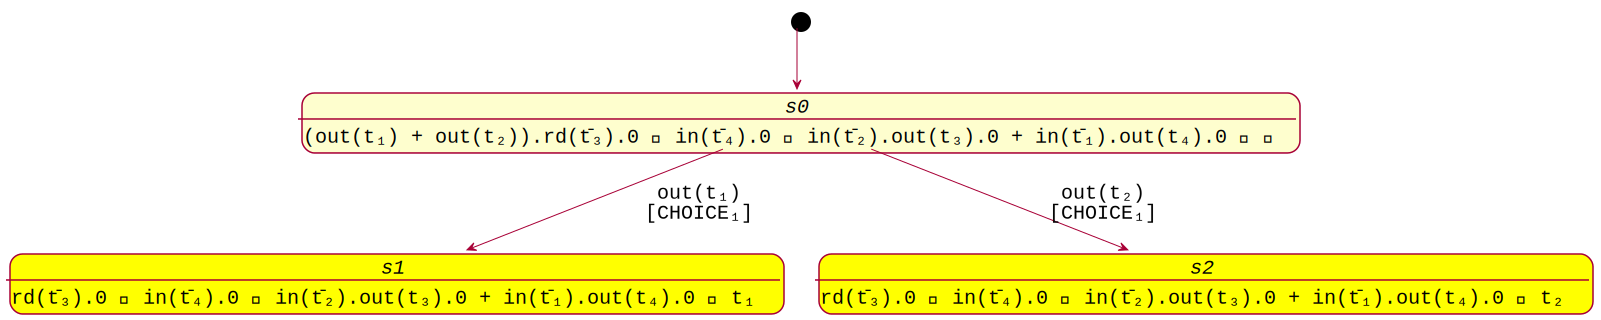
\includegraphics[width=\linewidth]{img/ex3.pdf}
    \end{center}
    
    \hint{Zoomable image \href{http://www.plantuml.com/plantuml/svg/lO_1JW8n48RlVOeviXB8mf4GGbmnUj43yOGS6ZfYGxVTj5CLZGSg9ho8R-DJx9EuiDeWuQgtQV_ld_-VeIDkoUUAkONK1RSyXpEyurxHkT4qbiy8tNHF71Cdt4cqL0YIk98pTznznNE4p7WhqR9xAH0mBsW90jtCoeAaqMpFwRQh0LuOm2cVBURMU2qoeupjzqTQI3qV3C0e-O37Y1kDJqKreQYe9Ifb7jahOvEJARHQ0t0fs-slXXuqZAS6bM6LG1E-vv0aRIiQzBakmrlIJg7SV83KzSVwy2CaxTfNiyqehA8GFUNcdRcqRj7fGSo-rPFiuleo6rMFQIIwaGW7nCy17VXzRG_-flUsP0pj_bzeO4FKmkVg2m00}{here}}

\end{frame}

\section{Dining Philosophers and Deadlocks}

\subsection{Simplifying Users}

\begin{frame}[allowframebreaks]
\frametitle{Let's further simplify Users}

     \begin{block}{From now on$\ldots$}
         \begin{itemize}
             \item We further simplify our formalism to keep the state graph in our examples \emph{small}
             \item Takeway: systems can be formalised at different \alert{level of detail}
         \end{itemize}
     \end{block}

     \bigskip

    \begin{enumerate}
        \item Imagine the syntax for users was simply defined as follows:
        %
        \[\begin{array}{rcl}
            U &::=& \mathtt{out}(T) \cdot U \mid \mathtt{in}(TT) \cdot U \\
            &\mid& \mathtt{rd}(TT) \cdot U \mid (U + U) \mid 0
        \end{array}\]
        
        \bigskip
        
        \item Then, imagine transition rule $[\text{COMPUTE}]$ and $[\text{COMPUTE}_i]$ where never defined, neither for $\mathcal{TS}$ nor for $\mathcal{CS}$
        
        \bigskip
        
        \item Then, imagine rule $[\text{IN}_i]$ was defined in the following way for $\mathcal{CS}$:
        %
        \[
    		\frac{
    			\mathtt{in}(\bar t) \cdot U_i \xrightarrow{\highlightG{?in(\bar t)}}_\mathcal{U} U_i 
    			\qquad
    			TS \cup t \xrightarrow{\highlightG{!in(t)}}_\mathcal{TS} TS
    			\qquad
    			t \in \bar{t}
    		}{
    			US \parallel \highlightR{\mathtt{in}(\bar t) \cdot U_i} \parallel US' \parallel \highlightB{TS \cup t}
    			\xrightarrow{\highlightG{in(t)}}_\mathcal{CS}
    			US \parallel \highlightR{U_i} \parallel US' \parallel \highlightB{TS}
    		}
    	\]
        
        \bigskip
        
        \item Finally, imagine rule $[\text{RD}_i]$ was defined in the following way for $\mathcal{CS}$:
        %
        \[
    		\frac{
    			\mathtt{rd}(\bar t) \cdot U_i \xrightarrow{\highlightG{?rd(\bar t)}}_\mathcal{U} U_i 
    			\qquad
    			TS \cup t \xrightarrow{\highlightG{!rd(t)}}_\mathcal{TS} TS \cup t
    			\qquad
    			t \in \bar{t}
    		}{
    			US \parallel \highlightR{\mathtt{rd}(\bar t) \cdot U_i} \parallel US' \parallel \highlightB{TS \cup t}
    			\xrightarrow{\highlightG{rd(t)}}_\mathcal{CS}
    			US \parallel \highlightR{U_i} \parallel US' \parallel \highlightB{TS \cup t}
    		} 
    	\]
    \end{enumerate}
\end{frame}

\subsection{Dining Philosophers Recap}

\begin{frame}
\frametitle{Dining Philosophers}
    \begin{columns}
        \begin{column}{.49\linewidth}
            \begin{itemize}
                \item $N$ philosophers are sitting on a round table spending their time \alert{eating} and \alert{thinking} 
                
                \item $N$ forks are on the table: philosopher $i$ has fork $i$ on his left and form $(i + 1) \mod N$ on his right
                
                \item In order to eat, philosopher $i$ must be holding \alert{both} fork $i$ and fork $(i + 1) \mod N$
                
                \item There is no way for a philosopher to take more than one fork \alert{at a time}
            \end{itemize}
        \end{column}
        \begin{column}{.49\linewidth}
            \includegraphics[width=\linewidth]{img/dining_pilosophers.png}
        \end{column}
    \end{columns}
\end{frame}

\startExercise

\subsection{Demo \currentExercise}

\begin{frame}[allowframebreaks]
\frametitle{Demo \currentExercise{} -- Three \href{https://en.wikipedia.org/wiki/Dining_philosophers_problem}{Dining Philosophers}, \emph{ordered}}
    
    Consider the system with \alert{$\mathtt{in}(\bar{t}_1) \cdot \mathtt{in}(\bar{t}_2) \cdot \mathtt{out}(t_1) \cdot \mathtt{out}(t_2) \cdot 0 \parallel \mathtt{in}(\bar{t}_2) \cdot \mathtt{in}(\bar{t}_3) \cdot \mathtt{out}(t_2) \cdot \mathtt{out}(t_3) \cdot 0 \parallel \mathtt{in}(\bar{t}_3) \cdot \mathtt{in}(\bar{t}_1) \cdot \mathtt{out}(t_3) \cdot \mathtt{out}(t_1) \cdot 0 \parallel t_1 \cup t_2 \cup t_3$}, where $t_i \in \bar{t}_i$ for all $i = 1,\ldots,3$, s.t. the \alert{ordered} \linda{} semantics defined before

    \bigskip

    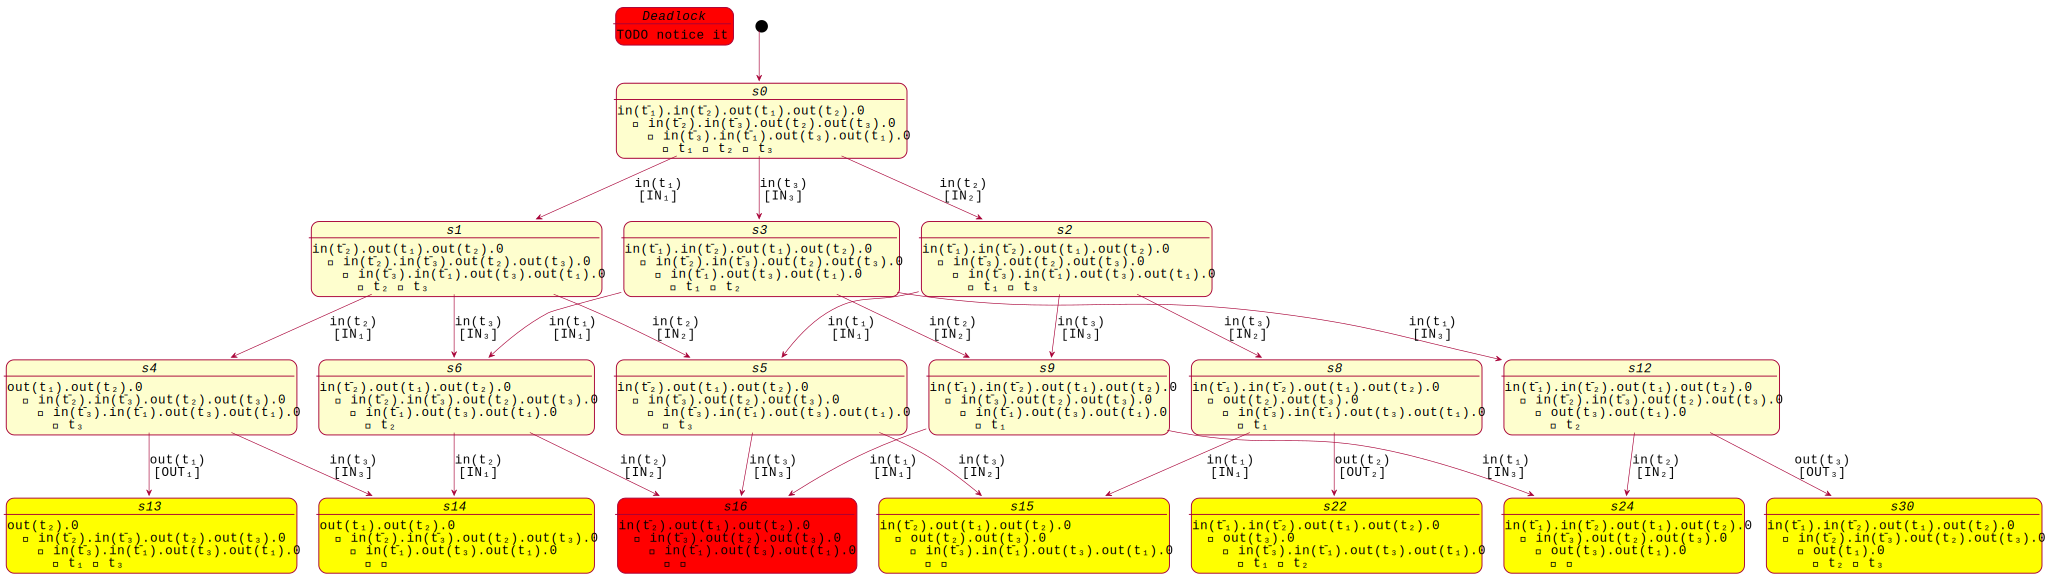
\includegraphics[width=\linewidth]{img/three_dining_philosophers.pdf}
    %
    \hint{SVG zoomable image available \href{http://www.plantuml.com/plantuml/svg/R8_1JW8n443l_OevWWbazKW8CO8cNk20di13inrnGhVTjBCg6W-21t_4Yz_YL_0bTgrDUjZRo_IzJkRSitJSL5huBPbQEbd13Ezbe_dA6bxI2y9PaJqkMJB-FV5E8n1BJQNlhkUoGfZQnX4wyK0A0QkQTw3Gbuvg9cj4LlhsQtWL01Uot6wSROoQMctTU7nf59dDP09MqoDs6JEKIjjo6no7gikuDVXS1q8Ld1rgRP_4cn1nQyeX_sa4DulP0enbAjjJXLYTtC5WC05Vn2x02CZq-EVZk7_l3nFk-qFRS8_3C54xAzO6uFZv1PcNy929YGx_IHP5CrkPr6nZYcBMZW9yjx1FS12-Y9USjWV4RcrMr_C0lyrNlMw6C0pSUOeymeVp8vAfRz2b7TdQjGjl0Efx5mbVJS6AcbQ134mdeRlpdJ7ZDqW0Pu2pW1RW0d0PE_ZIcsHQTEDWGhz9SQ9JJ03eDHC0Xfm9PFwHZlgHW0a4dKeI00uddRE0CMU2DPTNfBmNtMIv3YGkY1QWGRC8ODHo0XVSwa8h9U2nErPicHchUdvzsMG1Txdf-lAUrzRbcRTN8miqMzm0LGq4bVCPcBU-ge26N0Q7lpMntWxgfW6pqee5b2W92IHqfolMNhFbkYBceUa2IavGvGjA5oxENuQm9p1NSYQmVIHv8mQsbsRDptiicOQEf4LuEftdNQjWVJw5d3-HkwlH2hbmkAHlAgL2ZKZnhRXbrIvquNaCN-KbLsIYVUJ9rLzL-SF-wVtZRVsh_G80}{here}}
    
    \bigskip

    \begin{alertblock}{Consider state $s_{16}$}
        \begin{center}
            $s_{16} = \mathtt{in}(\bar{t}_2) \cdot \mathtt{out}(t_1) \cdot \mathtt{out}(t_2) \cdot 0 \parallel \mathtt{in}(\bar{t}_3) \cdot \mathtt{out}(t_2) \cdot \mathtt{out}(t_3) \cdot 0 \parallel \mathtt{in}(\bar{t}_1) \cdot \mathtt{out}(t_3) \cdot \mathtt{out}(t_1) \cdot 0 \parallel \emptyset$
        \end{center}
        %
        \begin{itemize}
            \item is it possible for the system to reach this state?
            \item what happens to the system when it reaches this state?
            \item is this the only critical state for the system?
        \end{itemize}
    \end{alertblock}

\end{frame}

\subsection{Deadlocks}

\begin{frame}
\frametitle{Aboud Deadlocks}
    \begin{block}{Deadlock}
        A situation where $N$ processes must access some shared resources in a mutually exclusive way and all of them get stuck, waiting for some other process to release a resource
    \end{block}
    
    \vfill
    
    \begin{alertblock}{Deadlock on a state graph}
        Deadlocks are those states on a state graph having \alert{no outgoing edge}, i.e., those states where \alert{no transition rule} can be applied (red states on the image)
    \end{alertblock}

\end{frame}

\begin{frame}
\frametitle{Demo \currentExercise{} -- Complete State Graph}

	\begin{figure}
		\centering
		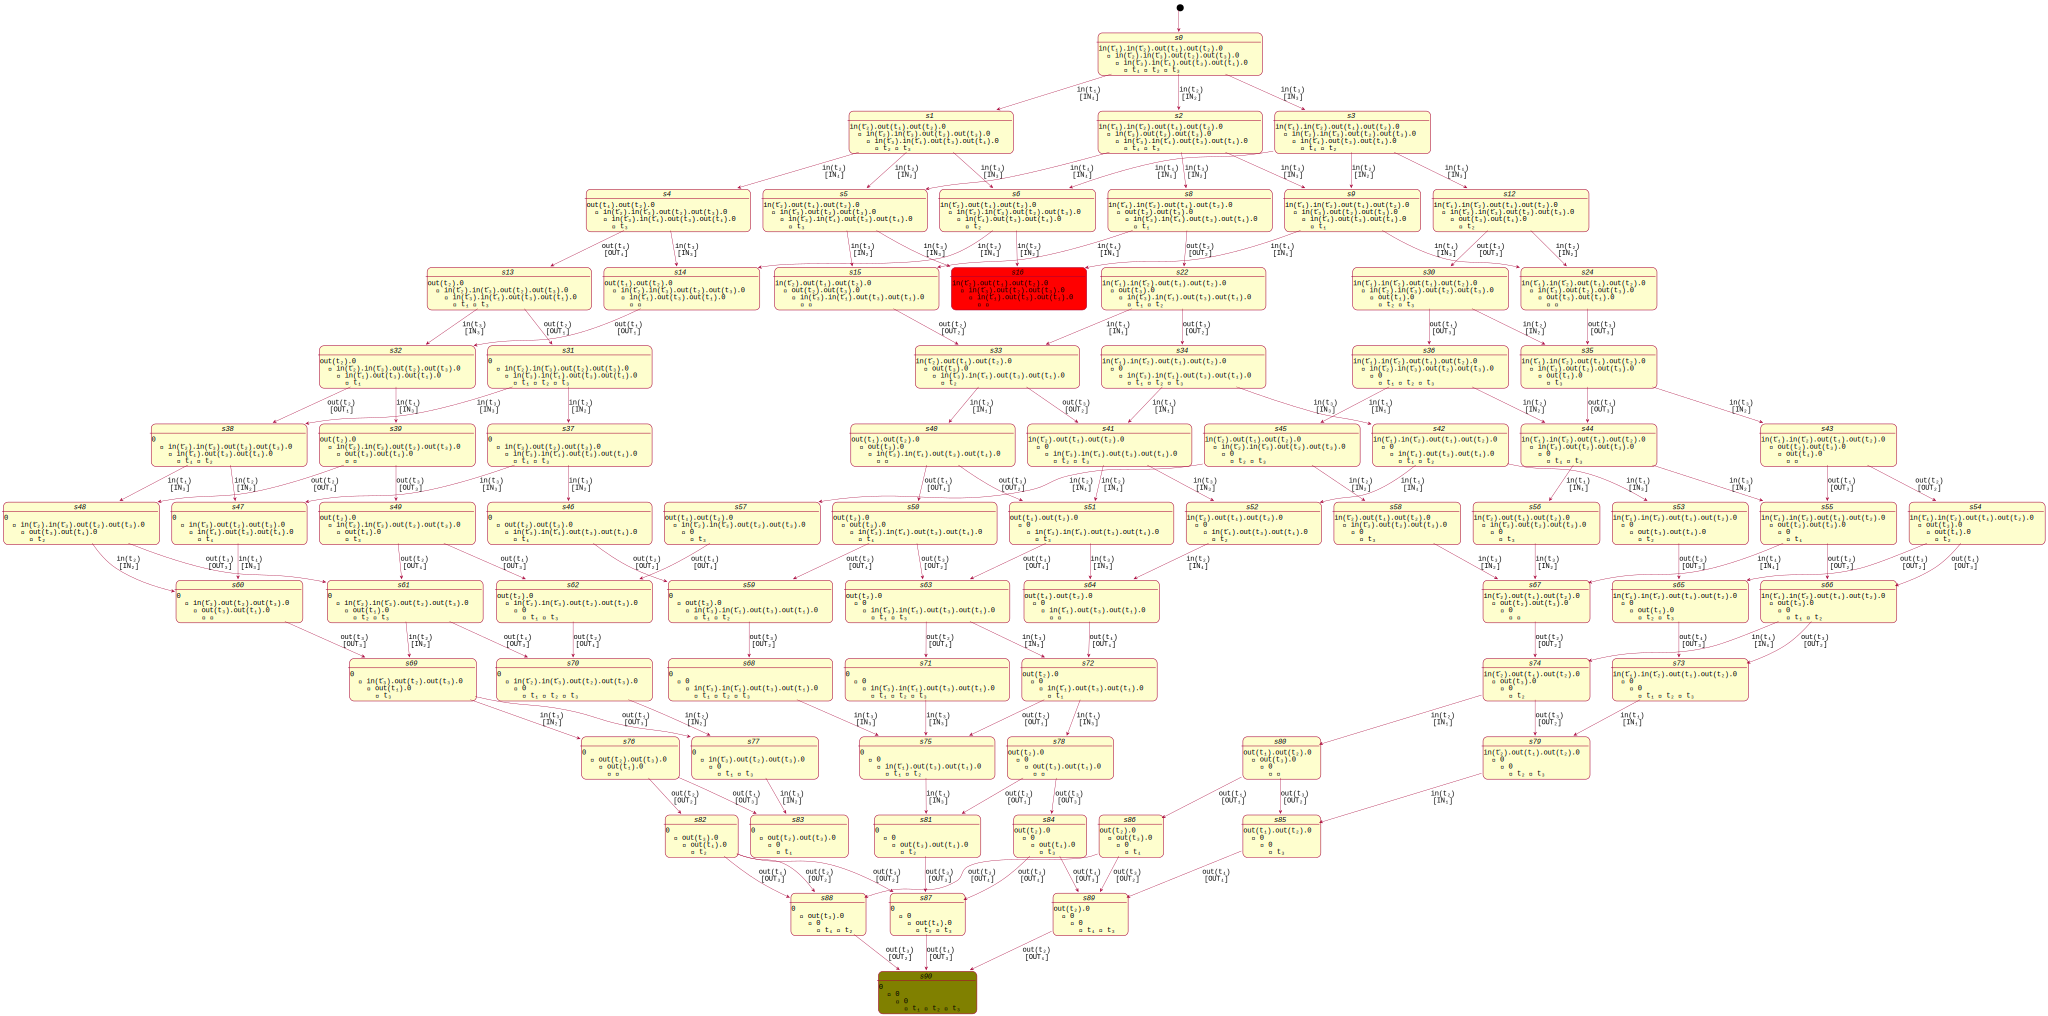
\includegraphics[width=.6\linewidth]{img/dining-philosophers-sol.pdf}
	\end{figure}
	%	
    \hint{Zoomable image available \href{http://www.plantuml.com/plantuml/svg/R90nJW9158RxESKhmGIoO4S8CO8cDZJ42YWcEq-SC3kpcNcheh5WryABs7WMJy59d0MURh7Tb_TzFs7sAf3qL6H6XAsskVGoWna-oCBGhREqqAy8mwGX5oG9Zufs1a6JD3eDxUkvp12chl0QlNZK2W6pd7QWCAHUvwIT5Orbg7yQtWJ0jKot6-yAgwREE3yUtrYbxMOo0MVq4xOLCvJAk7GR6u-ghRYt-997GXMR7HhZdiMx4CkBDVHw4mY9EFw122FGjaC_7uTot-qpbjs-AwX3zP4ftfAL1JXyVa6ZOwmQ8LDrdW2Fk6JSDrAc_Nd4i_eKuRk6ag4I8JczP50_uBHRsUNTFCBwJmvPbYpBVtd9ic9PhGL_bm6CuBTvQqTovOQ1-Jk5ZZ13WXzkv1iuiMzWfqxs3BwtnHAgHq5NYwQ6emrU1DHZ0mDq0r3j3yt6SnBsHoY6E8yam9X84c3CAWdXDbyTwqi2IGWU9wa46EiH9v80OrD9YBVhMcIwBtvzHs-7S6G1iS2QIOfWRAHEa0MxP-6dD85_TlE8eoFpg7x_yuyUrc4tzNNJH9ylZYivxiHA5bRPk1bHVRvGlJwpuwPK1MjMDLZdEd4T1_twhewRSG-i8Nm112hqAQvs5SsEnzKyBaOOi0Q3bIbek90u1ujm3q1EwWpck7tXVyG7GsYW787yQWdSeoFVIQdrJmQ7e7YZT-T7oUB-xzyxM0DOGks0YxRx40i0RdAuKVVvdc_Fi_iuzcMf1hGGfdfrHKLxguRWIJNIYxrPuH0PHo4mMyojOoKIpC4cpIpnmdriRCE86v0poeGvarP5O0zY-b7hOzmTUA5nmLpbRX26XM21ICS0Z9pquT24KAE1hcvutrjSc6oZWo7CEwS1137Nvmlhom2SZL0m1rbVQJ5xoKKa9iSOwIO2ixre_NmTfurzckp0-TGEiwbbfFF6nouUiJZ4JByCp4KLLwUDpvqhAY0o-eMvIkPgy_Gxf-En0HUdN3WqBVITxYvXMa0tL-gqyQ7wSD1K2qPRnAzw7B4T89bSm2nfrUQctNCgtm8WClQ1EQhAjxZY52BB9pekuqlEuP2q7DZgYLmHfvc3v8SDcEdj3H6anTSrsG398HRQ031N9LvTDowvZrbsE4slnZQdfXE0N1hp9jiBqhZu86KLS9WCmho_K9DpXL3St1i0SVs3Gz0ia3QA-FmAJ1kjG226GuvQzY2BgxGEz_yTWBXGmq7_iX4cP7hcify2u1160fpuhkQEmeaE9-cUINRUoKi3CWu8oWc7_A9dqWhHPpsJ752XAWbprgIUyeeJ9-kO3Bn2jbDPSDocS8hWmEUMg5VbfuxafpFa5PVTr1nDrOJRDN7PGJPl3aBkQG-Xk-BCcdVW8OC0p6LJ586IMtPB0Tm0F5HLWITIFASVH79qF3l7SpZ8nR1BsEb2YP8pG92qaETe_l-NN78yyKLDvVE4Kl52pex7gEh0hESqaDofqeXlM81HIb_djWkEpBawd2Ih6iH-tcquDt-PNo1XBhgsEdzSSF4j6-28hRZibtoqiezyjCAP_AtbjmIyp5aI3lBiMjuUvSVo51rC4p_mWYrEeIHdek9CNUblKZ2Nffcef_daus59ZcnN7wWtvHatlvBzjS3Pxd2G4lBekvClUQNWQJ7JbggwQ7nSB1Lvvvq31zFpP6bJMxdIyTBywQJsxph-WuDKmBhvQvbFCOT3qjtHK_d6cbztVwReXFVQVMDvhu4_WnQ0GzKjqEjqUYMdpz31enej-55PhuPmUPt3eRq8DurFqWn74iyyLtMcuGvdDIEhF5muIAf_v6j-4g_EPKrkTm-Oy_DrhNX5nz9q2MbUhWsloCsmRRUdFtNnk2R6XD_-_kUl-v_q_0S0}{here}}
    
    \begin{alertblock}{Consider the whole state graph}
        \begin{itemize}
            \item can the system terminate?
            \item will the system terminate in any possible scenario?
            \item does the system always terminate in a state where all processes are over?
        \end{itemize}
    \end{alertblock}

\end{frame}

\subsection{Analysing C/DS}

\begin{frame}%[allowframebreaks]
    \frametitle{Temporal Logics and Model Checking}

    \begin{itemize}
        \item Analysing the state graph of a C/DS let us not only \emph{debug} it but also \alert{proove} it is (in)correct
        
        \item Of course, generating and analysing the state graph by hand is not feasible, except for trivial cases
    \end{itemize}

    \vfill
    
    \begin{block}{Model Checking}
        \begin{itemize}
            \item Model checkers are tools capable of automatically inspecting a system's state graph
            \item They can check if a \alert{temporal logic} formula hold for the system or not
            \item[$\rightarrow$] Designers must express properties of interest via \alert{temporal logics}
        \end{itemize}
    \end{block}

    \vfill

    \begin{block}{Several sorts of temporal logics exist}
        \begin{itemize}
            \item[eg] Linear Temporal Logic (LTL), Computation Tree Logic (CTL)
            \item[!] we do not discuss them in this course 
        \end{itemize}
    \end{block}

\end{frame}

\section{Lab Activity}

\startExercise

\subsection{Writing Transition Rules}

\begin{frame}[allowframebreaks]
\frametitle{Exercise \currentExercise{} -- Writing Transition Rules}
    
    \begin{enumerate}
        \item<1-> Imagine the syntax for users was extended as follows:
        %
        \[\begin{array}{rcl}
            U &::=& \mathtt{out}(T) \cdot U \\
            &\mid& \mathtt{in}(TT) \cdot U \\
            &\mid& \mathtt{rd}(TT) \cdot U \\
            &\mid& \alert{\mathtt{no}(TT) \cdot U} \\
            &\mid& \alert{\mathtt{inp}(TT)\ ?\ U : U} \\
            &\mid& \alert{\mathtt{rdp}(TT)\ ?\ U : U} \\
            &\mid& \alert{\mathtt{nop}(TT)\ ?\ U : U} \\
            &\mid& (U + U) \mid 0
        \end{array}\]

        \bigskip
        
        \item Subject to the following axioms:
        %
        \[\begin{array}{rcl}
            (X\ ?\ T : F) \cdot Y &\equiv& X\ ?\ (T \cdot Y) : (F \cdot Y)
        \end{array}\]

        \framebreak

        \item Go on working on your local clone of the Lab \labN{} GitLab repository
        
        \bigskip
        
        \item Try extending the $\mathcal{CS}$ definition with new transition rules formally specifying the semantics of the \texttt{no}, \texttt{inp}, \texttt{rdp}, and \texttt{nop} primitives 
        
        \bigskip
        
        \item You can rely on the tools listed on slide \ref{useful-tools} for your exercise
        
        \bigskip
        
        \item Commit \& push your \texttt{README.md} file
        
    \end{enumerate}

\end{frame}

\begin{frame}
\frametitle{Exercise \currentExercise{} -- Example for the \texttt{nop} primitive}

    For instance, the \texttt{nop} primitive could be defined by means of the following transition rules:
    %
    \medskip
    %
    \[
		\frac{
			\forall t \in \bar{t} : TS \neq TS' \cup t
		}{
			US \parallel \highlightR{\mathtt{nop}(\bar t)\ ?\ U : U'} \parallel US' \parallel \highlightB{TS}
			\xrightarrow{\highlightG{nop(\bar t, \top)}}_\mathcal{CS}
			US \parallel \highlightR{U} \parallel US' \parallel \highlightB{TS}
		} 
		~[\text{NOP-T}_i]
	\]
	%
    \[
		\frac{
			\exists t \in \bar{t} : TS = TS' \cup t \quad 
		}{
			US \parallel \highlightR{\mathtt{nop}(\bar t)\ ?\ U : U'} \parallel US' \parallel \highlightB{TS}
			\xrightarrow{\highlightG{nop(\bar t, \bot)}}_\mathcal{CS}
			US \parallel \highlightR{U'} \parallel US' \parallel \highlightB{TS}
		} 
		[\text{NOP-F}_i]
    \]
    
    \medskip

    \begin{itemize}
        \item[!] notice the implicit definition of new sorts of events
    \end{itemize}

\end{frame}

\startExercise

\subsection{Formalising a System: the Coffee Machine}

    \begin{frame}[allowframebreaks]
    \frametitle{Exercise \currentExercise{} -- Formalising a System: the Coffee Machine}

    \begin{alertblock}{This is an \textbf{unconstrained} exercise}
        \begin{itemize}
            \item you are free to design your solution as you prefer
            \item no test is provided: testing is up to you
        \end{itemize}
    \end{alertblock}

    \bigskip

    \begin{alertblock}{This is a \textbf{mandatory} exercise}
        \begin{itemize}
            \item your solution will be inspected during lab activity verification
            \item you will be asked to discuss your solution
            \item collaboration and discussion with your colleagues (on the forum) is allowed
            \item asking for help on the forum is allowed
        \end{itemize}
    \end{alertblock}

    \bigskip
    
    \begin{enumerate}
        \item You must perform and end-to-end formalisation of a C/DS composed by a coffee machine and the user interacting with it
        
        \bigskip

        \item The system must take into account the following requirements:
        %
        \begin{itemize}

            \medskip
            
            \item Any coffee machine simply performs the following sort of actions:
            %
            \begin{itemize}
                \item it initially \alert{waits} for \alert{coins} to be inserted
                \item it then \alert{checks} if coins are sufficient
                \item it may optionally give \alert{change} back to the user
                \item it serves the \alert{coffee} to the user
                \item it finally \alert{waits} for the \alert{user} to take the coffee 
            \end{itemize}

            \medskip
            
            \item In turn, any user can perform the following actions:
            %
            \begin{itemize}
                \item he/she can \alert{walk} around
                \item he/she can \alert{chat} with some friends
                \item he/she can insert coins into the coffee machine in order to \alert{pay}
                \item it can \alert{take} the coffee the machine has eventually served
            \end{itemize}

            \medskip
            
            \item Of course, coffee machines can stop waiting for money only if some user pays 
            %
            Similarly, they can stop waiting for the coffee to be taken only if some user takes it
        \end{itemize}

        \bigskip
        
        \item Your formalisation must provide an interpretation and a semantics for the following formula:
        \\\vspace{.1cm}
        \alert{$
            s_0 = (\mathtt{chat} + \mathtt{walk}) \cdot \mathtt{insert} \cdot (\mathtt{walk} + \mathtt{chat}) \cdot \mathtt{take} \cdot 0
        $\\\hfill$    
            \quad\parallel
            \mathtt{waitCoin} \cdot \mathtt{check} \cdot (\mathtt{change} \cdot \mathtt{coffee} + \mathtt{coffee}) \cdot \mathtt{waitUser} \cdot 0
        $}

        \bigskip
        
        \item Draw the state graph of the system having $s_0$ as initial state, according to your semantics
        
        \bigskip
        
        \item You can rely on the tools listed on slide \ref{useful-tools} for your exercise
        
        \bigskip
        
        \item Commit \& push your \texttt{README.md} file
        
    \end{enumerate}
    

\end{frame}

\section{Useful tools}

\begin{frame}\label{useful-tools}
\frametitle{Useful tools}
    
    \begin{itemize}
        \item Web-based markdown editor supporting \LaTeX{} syntax for formulas
        %
        \begin{itemize}
            \item \url{https://upmath.me}
        \end{itemize}
        
        \vfill
        
        \item Web-based \href{http://plantuml.com/}{PlantUML} editor for designing State Charts (and other UML diagrams)
        %
        \begin{itemize}
            \item \href{http://www.plantuml.com/plantuml/uml/XOz1JW8n58RtFSLRWWbaW1qXG4HCt60Yi48MpVI93Prsqhwget4XmSG5rt2XPp7n3dCI2uYEoIGkclxfz_wlUNr7t99F57DBgLDkUG8dUCMzebEZQIpl4PfH0Ow94-uGPGf14bSoTkNj4KyG1iPRYPPTIu60IKeP27InbIb9ercXwRPgU600npnUBgpnMWoCChRJ6MeXzQBR1QFa3PPDJ3NUfI6X25CPAcLksIDZiwCvr6fTS17RwKDeW_5KeNprLAr_frMrBdM5FjQ_TmJvosiupyn5UqEZKBpKi_Ff9AGvEtW3_jUsUTksyyqxSuszjDc6ptMmdOt6mul9_EUzLR2LVDQ4lnkteTVh7M2h5FPH2v-eBm00}{\texttt{http://plantuml.com/plantuml}}
        \end{itemize}
        
        \vfill
        
        \item Web-based tool for converting \LaTeX{} formulas into Unicode strings
        %
        \begin{itemize}
            % \item \url{http://vikhyat.net/projects/latex_to_unicode}
            \item \url{https://www.unicodeit.net}
        \end{itemize}
    \end{itemize}
    
\end{frame}

\maketitle

%%%%%%%%%%%%%%%%%%%%%%%%%%%%%%%%%%%%%%%%%%%%%%%%%%%%%%%%%%%%%%%%%%%%%%%%%%%%%%%
\end{document}
%%%%%%%%%%%%%%%%%%%%%%%%%%%%%%%%%%%%%%%%%%%%%%%%%%%%%%%%%%%%%%%%%%%%%%%%%%%%%%%%
